\begin{frame}[t]{Überblick} 
    
    \begin{spacing}{0.9} \begin{tiny}
        \begin{minipage}{\textwidth}
          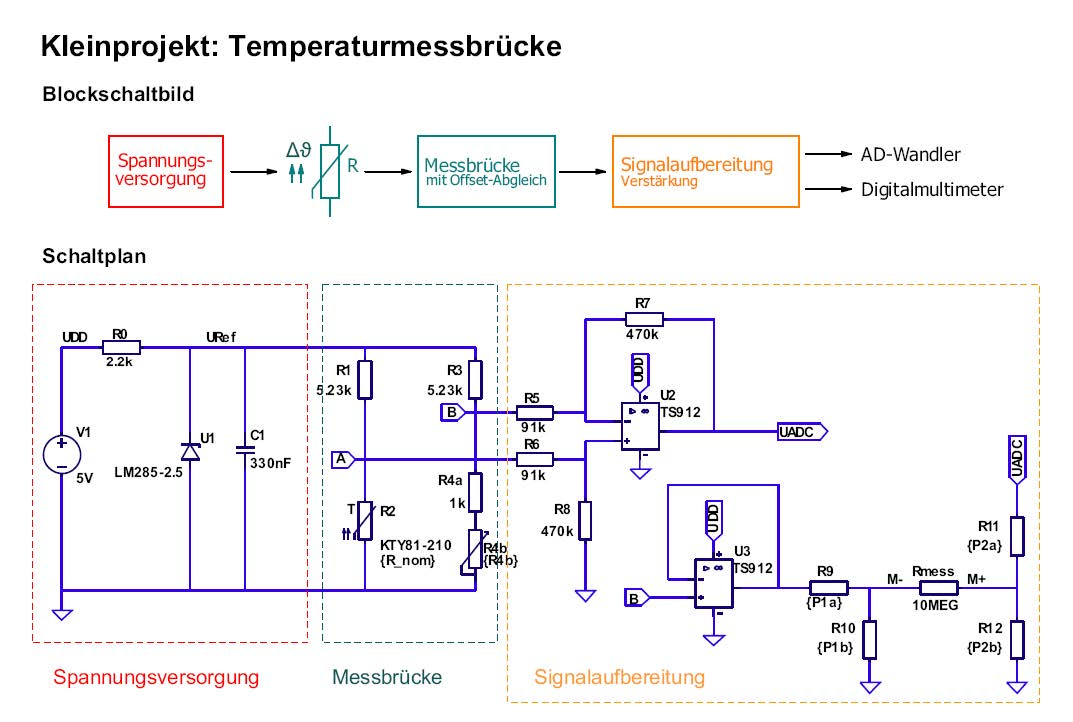
\includegraphics[width=\linewidth]{pictures/projekt_overview.jpg}
        \end{minipage} 
    \end{tiny} \end{spacing}

\end{frame}

\begin{frame}[t]{Vorgehenhensweise} 
    
    Zu diesem Zeitpunkt sollten wir alle in der Lage sein einfache Simulationen in DC-,AC-Sweep sowie transient
    durchführen zu können. Sie sollten den Bauteileditor sowie die grundlegenden Schematic-Funktionen (Rotate, Cut, \dots) 
    sicher beherrschen. 

    Wir werden nun die Bruecke und dir vorgestellten Bestandteile Stück für Stück aufbauen. 
    \textbf{Bitte beachtet Folgendes:}

    \begin{enumerate}
        \item Bitte speichern Sie alle Zwischenschritte ab, wir werden Teile später wiederverwenden
        \item Bei Fragen bitten wir Sie uns direkt im MS Teams zu benachrichtigen, sodass wir Ihren
        Fortschritt so gut wie möglich unterstützen können. 
    \end{enumerate}
\end{frame}

\begin{frame}[t]{Die Messbrücke - Arbeitspunktanalyse}  
    
    
    Die Grundlage für unsere Messbruecke bildet eine einfache Brückenschaltung. 
    Zur Wiederholung findet ihr unten den Schaltplan sowie die Formel zur Berechnung
    der Brueckenspannung. $V_{AB}$.

    
    \begin{table}[h!]
        \begin{tabular}{p{5cm} p{5cm}}
          \begin{minipage}{.5\textwidth}
            \begin{figure}
              \scalebox{0.6}{
            \centering
            \begin{circuitikz}
              \ctikzset{bipoles/thickness=1}
              \ctikzset{bipoles/length=.6cm}
              \draw
              (0,0) to [short, *-] (4,0)
              (0,0) to [V, l_=$V_{1}$] (0,-4)
              (2,0) to (2,-0.5) 
              (4,0) to (4,-0.5) 
              (2,-0.5) to [R, l_=$R_{1}$] (2,-1.5) 
              (2,-2.5) to [R, l_=$R_{2}$] (2,-3.5) 
              (2,-1.5) to (2,-2.5) 
              (2,-2) to [short,*-o] (2.25,-2) node[right]{$V_{a}$}
              (4,-1.5) to (4,-2.5) 
              (4,-2) to [short,*-o] (4.25,-2) node[right]{$V_{b}$}
              (4,-0.5) to [R, l_=$R_{3}$] (4,-1.5) 
              (4,-2.5) to [R, l_=$R_{4}$] (4,-3.5) 
              (2,-3.5) to (2,-4) 
              (4,-3.5) to (4,-4) 
              (0,-4) node[ground]{}
              (2,-4) node[ground]{}
              (4,-4) node[ground]{}
              ;
              \end{circuitikz} 
              }
              
          \end{figure}
          \end{minipage} 
          & 

        \begin{spacing}{0.9} \begin{tiny}
          \begin{minipage}{.5\textwidth}
          \begin{equation}
            V_{AB}=\frac{R_2R_3-R_4R_1}{(R_1+R_2)(R_3+R_4)}V_{1}
            \end{equation}
          \end{minipage} 
        \end{tiny} \end{spacing}
        \end{tabular}
      
      \end{table}

\end{frame}

\begin{frame}[t]{Die Messbrücke - Arbeitspunktanalyse} 
    
    \begin{spacing}{0.9} \begin{tiny}
    \begin{table}[h!]
      \begin{tabular}{p{3cm} p{7cm}}
        \hline
        \textbf{Simulation \& Analyse} & \\
        \hline \\
        \begin{minipage}{.3\textwidth}
         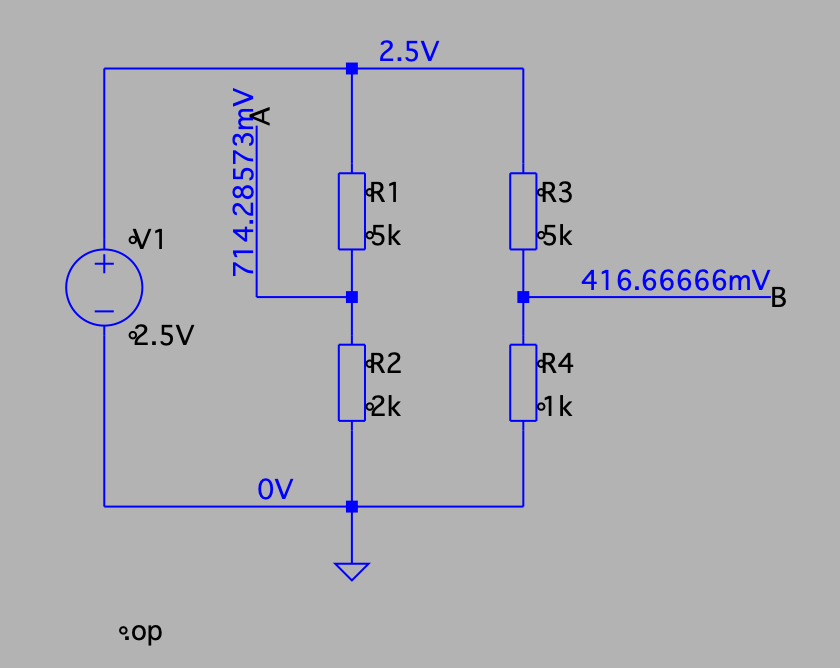
\includegraphics[width=\linewidth]{pictures/bridge_op_1.png}
       \end{minipage} 
       & 
       \begin{minipage}{.7\textwidth}
       \begin{itemize}
         \item tbd
       \end{itemize}
       \end{minipage} 
       \\
      \end{tabular}
    \end{table}
  \end{tiny} \end{spacing}
  

     \end{frame}